\section{Neuronale Netze}

Ein neuronales Netz besteht aus mehreren Schichten von Neuronen. Die wichtigsten Schichten sind die Eingabeschicht, eine oder mehrere versteckte Schichten (Hidden Layers) und die Ausgabeschicht.

\subsection*{Aufbau eines Neurons}

Jedes Neuron in einer Schicht ist mit den Neuronen der vorherigen Schicht verbunden. Jede dieser Verbindungen hat ein Gewicht \( w \), das die Stärke der Verbindung angibt. Zusätzlich hat jedes Neuron einen Bias \( b \), der als Schwellenwert dient.

Die Berechnung in einem Neuron erfolgt in zwei Schritten:

\begin{enumerate}
    \item \textbf{Lineare Kombination:} Zuerst wird eine gewichtete Summe der Eingaben gebildet:
    \[
    z = \sum_{i=1}^{n} w_i \cdot x_i + b
    \]
    Hierbei sind \( x_i \) die Eingaben, \( w_i \) die Gewichte und \( b \) der Bias.

    \item \textbf{Aktivierungsfunktion:} Anschließend wird das Ergebnis \( z \) durch eine Aktivierungsfunktion \( \sigma \) transformiert, um die Ausgabe des Neurons zu berechnen:
    \[
    h = g(z)
    \]

\end{enumerate}

\begin{figure}[h]
    \centering
    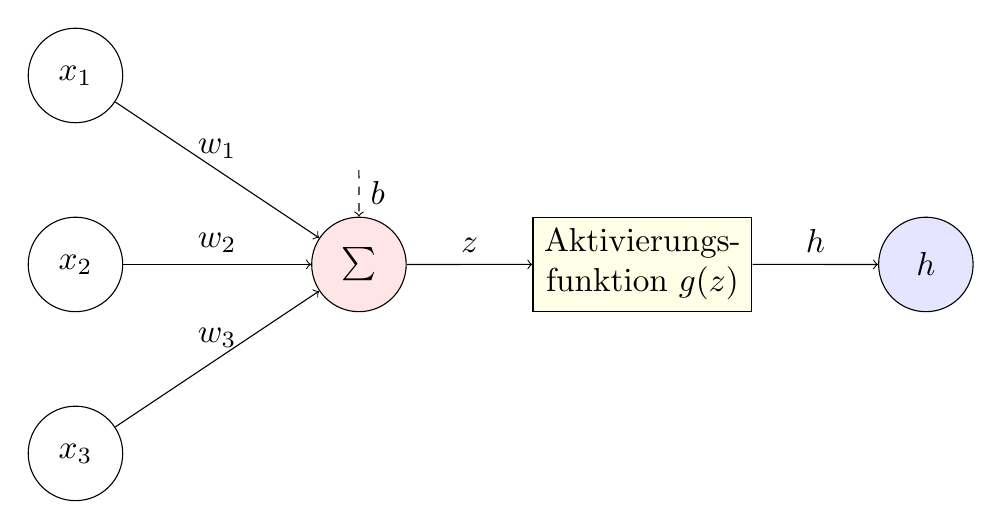
\begin{tikzpicture}[scale=1.2, transform shape]
        % Eingaben
        \node[circle, draw, minimum size=1cm] (I1) at (0, 2) {$x_1$};
        \node[circle, draw, minimum size=1cm] (I2) at (0, 0) {$x_2$};
        \node[circle, draw, minimum size=1cm] (I3) at (0, -2) {$x_3$};

        % Neuron
        \node[circle, draw, minimum size=1cm, fill=red!10] (N) at (3, 0) {$\sum$};

        % Aktivierungsfunktion Block
        \node[draw, minimum size=1cm, fill=yellow!10, align=center] (A) at (6, 0) {Aktivierungs-\\funktion $g(z)$};

        % Ausgang
        \node[circle, draw, minimum size=1cm, fill=blue!10] (O) at (9, 0) {$h$};

        % Verbindungen
        \draw[->] (I1) -- (N) node[midway, above] {$w_1$};
        \draw[->] (I2) -- (N) node[midway, above] {$w_2$};
        \draw[->] (I3) -- (N) node[midway, above] {$w_3$};
        \draw[->] (N) -- (A) node[midway, above] {$z$};
        \draw[->] (A) -- (O) node[midway, above] {$h$};

        % Bias
        \draw[->, dashed] (3, 1) -- (N) node[midway, right] {$b$};

    \end{tikzpicture}
    \caption{Einzelnes Neuron mit Gewichten, Bias und Aktivierungsfunktion.}
    \label{fig:single_neuron}
\end{figure}

\begin{figure}[h]
    \centering
    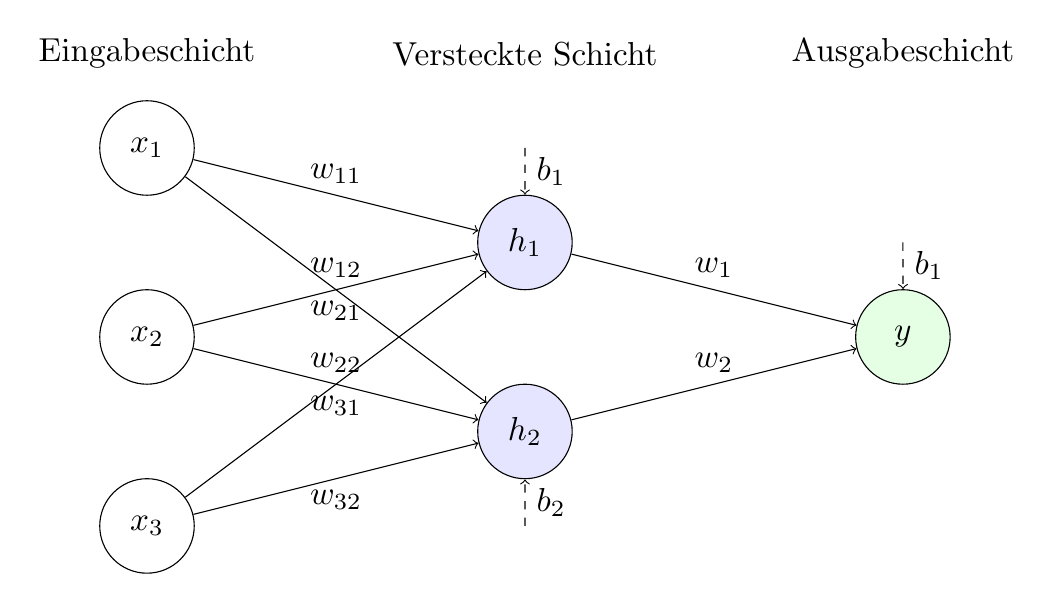
\begin{tikzpicture}[scale=1.2, transform shape]
        % Neuronen der Eingabeschicht
        \node[circle, draw, minimum size=1cm] (I1) at (-1, 2) {$x_1$};
        \node[circle, draw, minimum size=1cm] (I2) at (-1, 0) {$x_2$};
        \node[circle, draw, minimum size=1cm] (I3) at (-1, -2) {$x_3$};
        \node[draw=none] at (-1, 3) {Eingabeschicht};

        % Neuronen der versteckten Schicht
        \node[circle, draw, minimum size=1cm, fill=blue!10] (H1) at (3, 1) {$h_1$};
        \node[circle, draw, minimum size=1cm, fill=blue!10] (H2) at (3, -1) {$h_2$};
        \node[draw=none] at (3, 3) {Versteckte Schicht};

        % Neuronen der Ausgabeschicht
        \node[circle, draw, minimum size=1cm, fill=green!10] (O1) at (7, 0) {$y$};
        \node[draw=none] at (7, 3) {Ausgabeschicht};

        % Eingabeschicht zu versteckte Schicht
        \draw[->] (I1) -- (H1) node[midway, above] {$w_{11}$};
        \draw[->] (I1) -- (H2) node[midway, above] {$w_{12}$};
        \draw[->] (I2) -- (H1) node[midway, below] {$w_{21}$};
        \draw[->] (I2) -- (H2) node[midway, above] {$w_{22}$};
        \draw[->] (I3) -- (H1) node[midway, below] {$w_{31}$};
        \draw[->] (I3) -- (H2) node[midway, below] {$w_{32}$};

        % Versteckte Schicht zu Ausgabeschicht
        \draw[->] (H1) -- (O1) node[midway, above] {$w_{1}$};
        \draw[->] (H2) -- (O1) node[midway, above] {$w_{2}$};

        % gehe vom knoten nach oben und setze da den pfeil senkrecht nach unten mit der beschriftung
        \draw[->, dashed] (3, 2) -- (H1) node[midway, right] {$b_1$};
        \draw[->, dashed] (3, -2) -- (H2) node[midway, right] {$b_2$};
        \draw[->, dashed] (7, 1) -- (O1) node[midway, right] {$b_1$};
        
    \end{tikzpicture}
    \caption{Ein einfaches neuronales Netz mit einer Eingabeschicht, einer versteckten Schicht und einer Ausgabeschicht.}
    \label{fig:neural_network}
\end{figure}



Die Eingabeschicht besteht aus Neuronen, die die Daten ins Netz einspeisen. In der Grafik sind dies \( x_1 \), \( x_2 \) und \( x_3 \). Diese Neuronen nehmen die Rohdaten auf, die das Netz verarbeiten soll, dies können z.B. Sample Werte eines digitalen Signals sein.

Die versteckte Schicht (oder Hidden Layer) verarbeitet die Eingaben aus der Eingabeschicht. In der Grafik sind dies die Neuronen \( h_1 \) und \( h_2 \). Diese Schicht führt Berechnungen durch, um Muster und Merkmale in den Daten zu erkennen.

Die Ausgabeschicht liefert das Endergebnis des neuronalen Netzes. In der Grafik ist dies das Neuron \( y \). Dieses Neuron gibt z.B. die Wahrscheinlichkeit aus, dass ein Bild eine Katze zeigt.


\subsection{Aktivierungsfunktionen}

Aktivierungsfunktionen helfen einem neuronalen Netz, komplexe Muster in den Daten zu erkennen. Hier sind vier wichtige Aktivierungsfunktionen, die oft verwendet werden:

\begin{enumerate}
    \item \textbf{Sigmoid-Funktion:} 
    $$
    \sigma(z) = \frac{1}{1 + e^{-z}}
    $$
    Diese Funktion gibt Werte zwischen 0 und 1 aus.
    
    \item \textbf{Tanh-Funktion:}
    $$
    \tanh(z) = \frac{e^z - e^{-z}}{e^z + e^{-z}}
    $$
    Diese Funktion gibt Werte zwischen -1 und 1 aus.
    
    \item \textbf{ReLU-Funktion:}
    $$
    \mathrm{ReLU}(z) = \max(0, z)
    $$
    Diese Funktion gibt 0 aus, wenn \(z\) negativ ist, und \(z\), wenn \(z\) positiv ist.
    
    \item \textbf{Lineare Funktion:}
    $$
    g(z) = z
    $$
    Diese Funktion gibt den Eingabewert direkt aus.
\end{enumerate}

\begin{figure}[h]
    \centering
    \includegraphics[width=0.8\textwidth]{images/activation_functions.pdf}
    \caption{Verschiedene Aktivierungsfunktionen: Sigmoid, Tanh, ReLU und Linear.}
    \label{fig:activation_functions}
\end{figure}

\subsection{Training eines neuronalen Netzes}



\subsection{Training mit der ANT-GUI}

Die grafische Benutzeroberfläche ermöglicht es, ein neuronales Netz zu trainierren, dass die Samples eines OOK-Signals klassifiziert. Dazu wird ein Datensatz benötigt, der die Samples des Signals enthält. Dieser Datensatz wird in zwei Teile aufgeteilt: einen Trainingsdatensatz und einen Testdatensatz. Der Trainingsdatensatz wird verwendet, um das neuronale Netz zu trainieren, während der Testdatensatz verwendet wird, um die Genauigkeit des Netzes zu überprüfen.
Der Startbildschirm der Oberfläche ist in Abbildung \ref{fig:ant_gui} zu sehen. Ein OOK Symbol besteht aus 100 Samles, was im Netzwerk als 100 Eingaben interpretiert wird. 


\begin{figure}[h]
    \centering
    \includegraphics[width=0.75\textwidth]{images/GUI_start.png}
    \caption{Die ANT-GUI mit einem trainierten neuronalen Netz.}
    \label{fig:ant_gui}
\end{figure}

\begin{aufgabe}
    Trainiere ein neuronales Netz, bei dem die Genauigkeit mindesten 90\% beträgt und speichere das Modell ab.
\end{aufgabe}

\begin{lösung}
    Die Ergebnisse hängen nicht von der Tiefe und Komplexität des Netzwerks ab, sondern vor allem von der gewählten Kostenfunktion und den Aktivierungsfunktionen.
\end{lösung}

Ein beispielhaftes Netzwerk, wie es in der GUI angezeigt wird, ist in Abbildung \ref{fig:gui_network} zu sehen.

\begin{figure}[h]
    \centering
    \includegraphics[width=0.8\textwidth]{images/GUI_network.png}
    \caption{Ein beispielhaftes neuronales Netz in der ANT-GUI.}
    \label{fig:gui_network}
\end{figure}

Das Netwerk besitzt 3 versteckte Schichten mit je 5 Neuronen pro Schicht. Die Eingabeschicht hat 100 Neuronen, die die Samples des OOK-Signals repräsentieren. Die Ausgabeschicht hat 1 Neuron, das die Wahrscheinlichkeit ausgibt, dass das Signal eine 1 bzw. eine 0 ist.


\section{OOK Erkennung mit einem neuronalen Netz in Gnuradio}

GNU Radio ist eine Open-Source-Software, die es ermöglicht, Radiosignale auf einem Computer zu verarbeiten. Mit GNU Radio kann man verschiedene Funksignale empfangen, analysieren und senden, indem man Module und Bausteine zu einem Signalverarbeitungssystem zusammenfügt.

Ein RTL-SDR (Software Defined Radio) ist ein günstiger USB-Stick, der ursprünglich als TV-Tuner entwickelt wurde, aber auch verwendet werden kann, um Funksignale aus der Umgebung zu empfangen. Mit diesen beiden Tools können wir ein OOK-Signal empfangen und mit einem konventioneller Signalverarbeitung oder einem neuronalen Netz erkennen.





